% FIGURE 1 --- conceptual overview. Three stages acting on THE SAME successor
% set, so the reader sees three layers on one molecular graph, not three methods.
%
% STATUS: drawn and installed as figures/fig1_overview.png.
% NOT YET CARRIED BY THE INSTALLED ARTWORK, both flagged deliberately:
%   - the A(x) -> S(x) two-layer structure and the two-marks-merge-to-one-
%     successor detail. The installed figure draws x straight to the y_i.
%   - the +1 / -1 / 0 / ring badges. Since the caption no longer says
%     "including cardinality- and topology-changing transitions", nothing
%     in the paper currently states that the edits change atom count.
% Source at 1672x941 = 304 ppi at \textwidth. Above the 300 print floor but
% well under the ~600-1100 ppi of the comparison figures.
% ===================== DRAWING SPEC =====================
%
% IDENTITY. The formal figure title is "Overview of COMPOSE", not a slogan.
% POSSIBLE / PLAUSIBLE / PURPOSEFUL stay as the visual organizing motif inside
% the panels, paired with the technical object each one names, so a reviewer
% sees immediately what the word refers to. Do not promote the mnemonic to the
% caption headline.
%
% THE ONE MATHEMATICAL CORRECTION. The previous sketch drew
%     x --A(x)--> {y_1,...,y_m}
% which conflates Sec. 4.1 with Sec. 4.3. A(x) is a set of EDIT MARKS; the y_i
% are CANONICAL MOLECULAR SUCCESSORS. Draw the two as distinct layers:
%     x  ->  A(x) [legal edit marks]  ->  S(x) [distinct molecular successors]
% and draw at least TWO symmetry-equivalent marks converging on the SAME y_i.
% That single visual detail explains canonicalization (Sec. 4.3) with no prose,
% and mirrors the worked example already in the text: deleting any of the three
% equivalent terminal methyls of 2-methylpropane gives propane once, carrying
% the combined probability of those marks.
%
% CHOICE OF x. Take a real molecule from an audited executor fiber, not an
% invented schematic. Source: docs/GENMOL_T4_SEEDS.json, whose full fibers were
% enumerated in diagnostics/compose_delta_n_audit.json (10,199 applied
% successors, 8 executor families, heavy-atom delta distribution
% {-1: 95, 0: 5964, +1: 4140}, zero |delta n| > 1). Pick one on the small side
% so five successors are legible at column width.
%
% THE FIVE SUCCESSORS. Representative, not exhaustive. One per row of the
% audited family table:
%     +1  atom_insert          (birth)
%     -1  atom_delete          (death)
%      0  atom_restate_semantic or bond_reorder   (same cardinality)
%      0  bond_reroute         (topology change, cardinality fixed)
%      0  cycle_close or cycle_open               (ring change, if legible)
% Five is plenty. Do not draw all eight families.
%
% PANEL INVARIANCE IS THE WHOLE POINT. Panels (a), (b), (c) must show the SAME
% x, the SAME y_i, in the SAME screen positions. Only the arrow weights change
% between them. A reader who glances for five seconds should conclude: COMPOSE
% did not change what is possible, it learned how probability is distributed
% over what is possible, and then reweighted that by purpose.
%
%   (a) all arrows EQUAL weight. No probabilities yet.
%   (b) arrow width = R_theta(y|x). Tag the panel "goal-independent".
%   (c) arrow width = P_phi(y|x,z,b). For two or three successors, faint
%       continuation trees to the right showing y_i -> ... -> desirable future.
%       Without those trees h_phi reads as just another local scorer; with them
%       the picture teaches that a locally ordinary edit is upweighted because
%       of what remains REACHABLE from it. Draw z and b entering the controller
%       ONLY, never R_theta.
%
% THE CAPTION IS DELIBERATELY SHORT (~65 words), matching the TD3B three-panel
% overview rather than a five-panel workflow figure. It decodes the mathematical
% object in each panel and nothing more. Two things were therefore CUT from the
% caption and are now the DRAWING's job. If the figure does not carry them, the
% information is lost from the paper entirely:
%
%   1. "including cardinality- and topology-changing transitions" -- panel (a)
%      must make birth (+1), death (-1) and topology change visibly obvious from
%      the drawn successors themselves.
%   2. "across objectives the support and R_theta remain fixed; purpose enters
%      through the controller" -- panel (c) must show z and b entering ONLY the
%      controller, with R_theta visibly persisting underneath unchanged.
%
% Division of labour: the FIGURE tells the conceptual story (possible ->
% plausible -> purposeful); the PANEL HEADINGS name the sober technical objects;
% the CAPTION decodes the three panels. The caption is not a mini-abstract.
%
% ===================== VISUAL STYLE TARGET =====================
% Reference figures: BranchedSBM Fig 1, EntangledSBM Fig 1, PepTune Fig 2.
% These are the Chatterjee-lab house style and are what this figure should look
% like. Extracted rules (hex values are eyeballed from the references and are
% approximate, but the ROLES are the point):
%
%  1. NESTED ROUNDED CONTAINERS. A very pale lavender rounded rectangle wraps
%     the whole figure (~#F7F0FB); each panel is a nested white or near-white
%     rounded card with a hairline border. PepTune nests two levels deep.
%     Generous internal padding. No hard rectangles anywhere.
%
%  2. ONE HUE FAMILY. Everything lives on a blue -> indigo -> magenta ramp.
%     Nothing falls outside it; there is no second accent colour.
%       deep navy    ~#1B1B8F   equation boxes, panel letters, headings
%       indigo       ~#6B6BD6   primary nodes, primary arrows
%       cyan/teal    ~#4EC3E0   secondary branch
%       orchid       ~#C46BD6   tertiary branch
%       tints of the above at 10-20% for fills and density clouds
%
%  3. THE SIGNATURE MOVE: primary equations sit in FILLED DEEP-NAVY ROUNDED
%     BOXES WITH WHITE TEXT. Secondary/annotation equations sit in WHITE
%     rounded boxes with a THIN BORDER IN THE BRANCH'S OWN COLOUR. This is the
%     single most recognisable element of the style, and the current COMPOSE
%     draft does not do it -- the P_phi equation is in a pale lavender box and
%     should be navy-filled with white text.
%
%  4. PANEL LETTERS are large, bold, navy, top-left of each panel card.
%
%  5. MOLECULES AS NODE-LINK GRAPHS: filled circles of varying radius in the
%     palette colours, thin bonds, no atom labels. EntangledSBM Fig 1 is the
%     model. The current draft already does this correctly.
%
%  6. ARROWS are curved, with width carrying magnitude, and often a large
%     sweeping arc for the outer loop. Dashed for "not yet weighted" or for
%     conditioning inputs, solid for committed flow.
%
%  7. Sans-serif labels, lots of whitespace, no gridlines, no chart junk.
%
%  8. Caption below the frame: "Figure N: <bold title>." then plain prose.
%
% FORMAT. The references are vector. A raster export will look blurry next to
% them in the proceedings, so this figure must ship as PDF or SVG, never PNG.
% If it cannot be exported as vector from the design tool, build it in TikZ.
%
% DELIBERATELY OMITTED. No retargeting inset. The old "z_A -> x_3 -> z_B" was
% also semantically wrong (z_A does not transition into x_3, and x_3 does not
% transition into z_B). Retargeting lands far better in Sec. 4.8 and Sec. 5.5,
% once the reader already understands that x_3 is a real reusable molecular
% state. Figure 1 carries one architecture: executor -> canonical successors ->
% reference process -> future-aware control. That is enough.
% ==============================================================================
\begin{figure}[t]
\centering
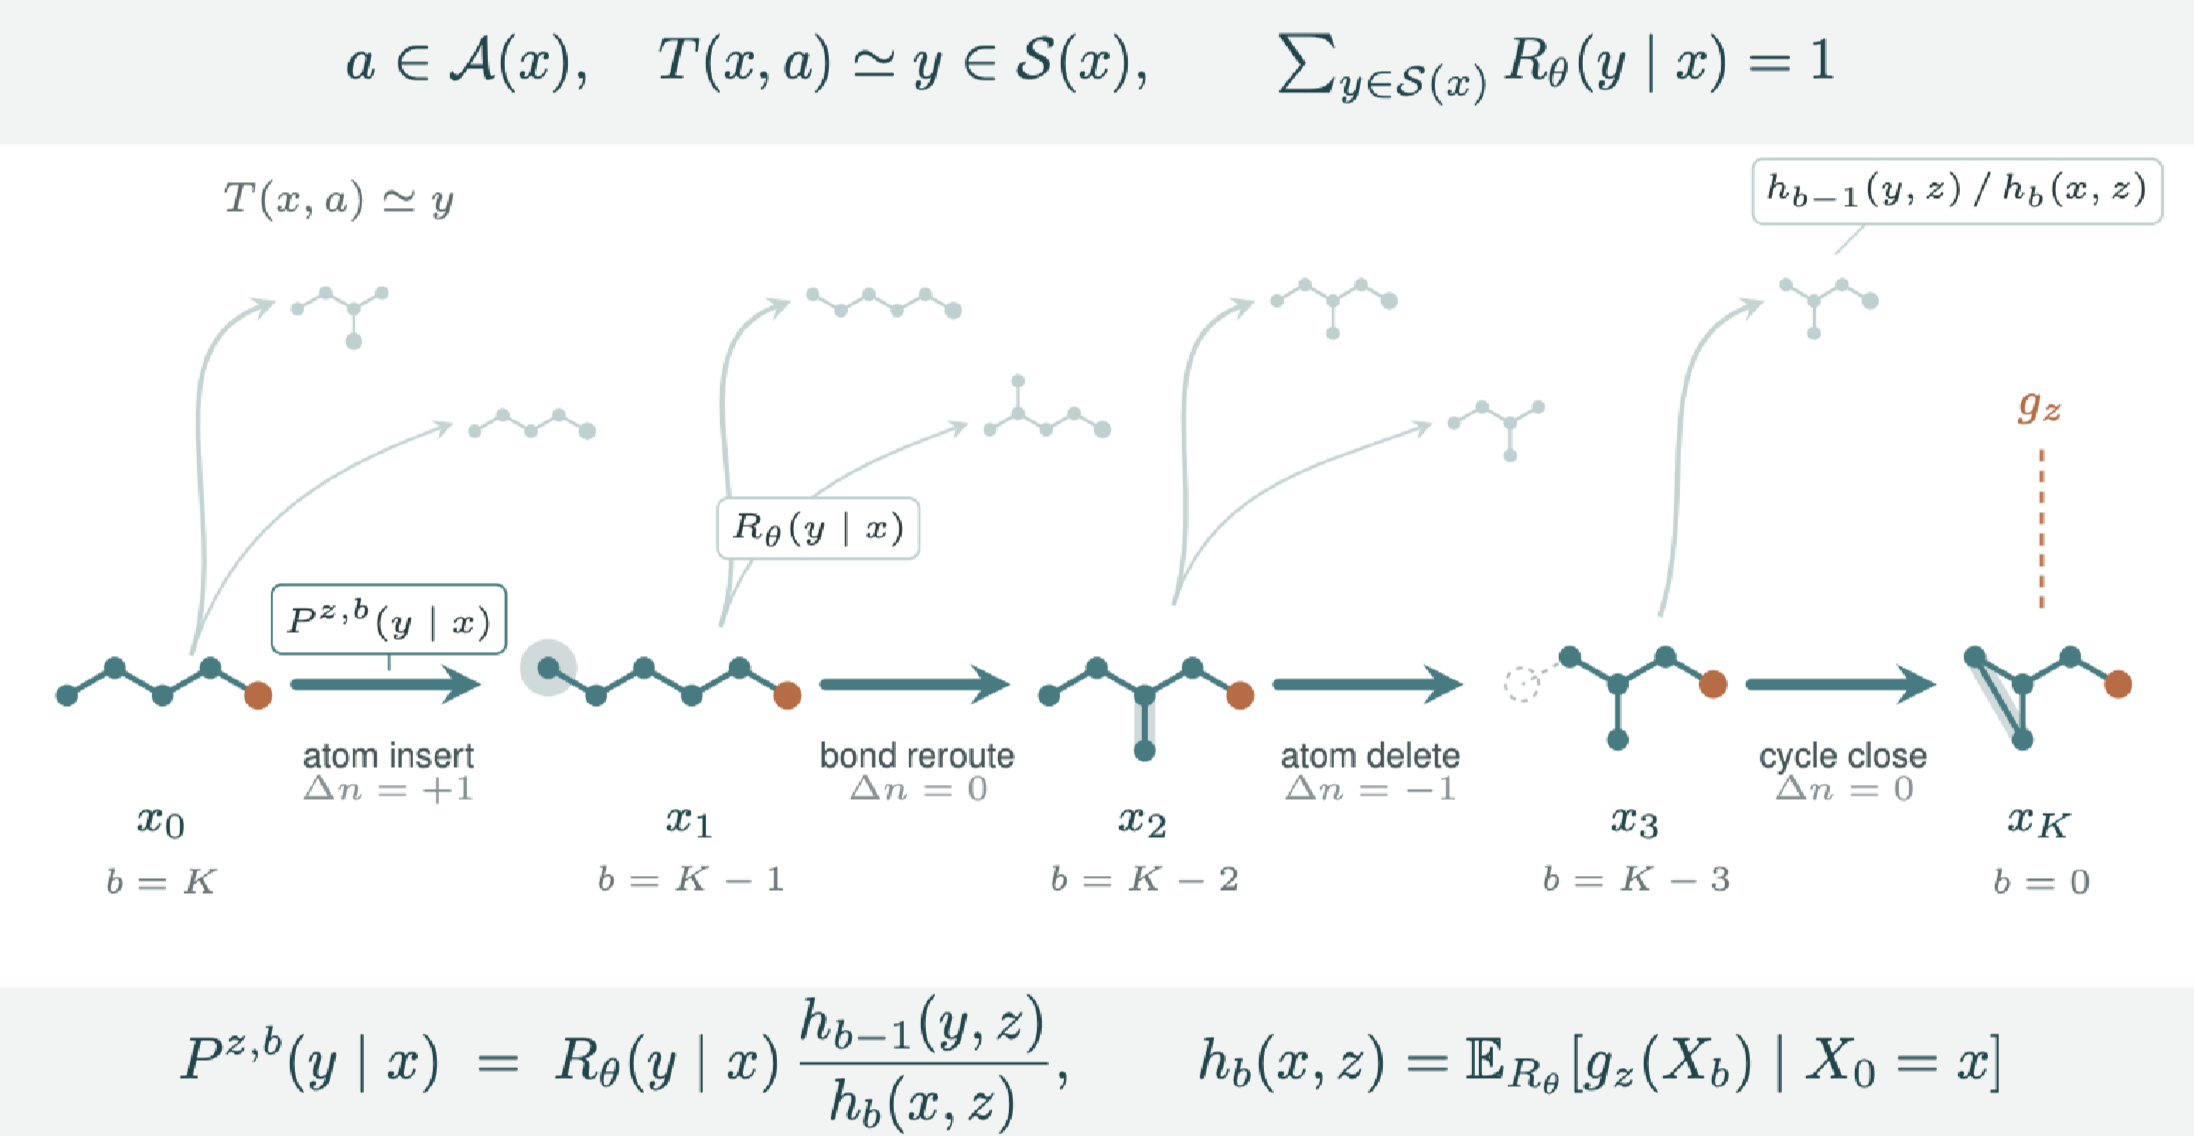
\includegraphics[width=\textwidth]{figures/fig1_overview.png}
\caption{\small Overview of COMPOSE. From a molecule \(x\), the graph-rewrite
executor admits edit marks \(a\in\mathcal A(x)\), which induce distinct canonical
successors \(y\in\mathcal S(x)\). The goal-independent reference kernel
\(R_\theta(y\mid x)\) assigns probability over this executable successor set, and
iterating \(R_\theta\) defines a trans-dimensional process over complete molecules.
For objective \(z\) and \(b\) remaining edits, finite-horizon control reweights each
reference transition by its remaining future value,
\(P^{z,b}(y\mid x)=R_\theta(y\mid x)h_{b-1}(y,z)/h_b(x,z)\), with
\(h_b(x,z)=\mathbb E_{R_\theta}[g_z(X_b)\mid X_0=x]\). Control therefore changes
which executable molecular transitions are preferred without introducing
transitions outside the support of \(R_\theta\).}
\label{fig:ppp}
\end{figure}
